\documentclass[../main]{subfiles}
\begin{document}
\chapter{Tablas y Problemas Resueltos}
\section{Problemas Resueltos}

\subsection{Electromagnetismo T.P.N.\textsuperscript{o}:1}

Usando el cuadro 1 determinar la permeabilidad relativa $\mu_r$ para hierro forjado expuesto a intensidades de campo $H = \qty{120}{Av/m}$, $H = \qty{2400}{Av/m}$, $H = \qty{27000}{Av/m}$ y $H = \qty{580}{Av/m}$.

\begin{align*}
B &= \mu H \Rightarrow \mu = \frac{B}{H} & \mu_r &= \frac{\mu}{\mu_0}
\end{align*}

\begin{align*}
\mu_{120} &= \frac{\qty{0,3}{T}}{\qty{120}{Av/m}} = \boxed{\qty{0,0025}{Tm/Av}} & \mu_{r120} &= \frac{0,0025}{4\pi \times 10^{-7}} = \boxed{1989,44} \\
\mu_{2400} &= \frac{\qty{1,5}{T}}{\qty{2400}{Av/m}} = \boxed{\qty{0,000625}{Tm/Av}} & \mu_{r2400} &= \frac{0,000625}{4\pi \times 10^{-7}} = \boxed{497,36} \\
\mu_{27000} &= \frac{\qty{2}{T}}{\qty{27000}{Av/m}} = \boxed{\qty{0,0000741}{Tm/Av}} & \mu_{r27000} &= \frac{0,0000741}{4\pi \times 10^{-7}} = \boxed{58,97} \\
\mu_{580} &= \frac{\qty{1,1}{T}}{\qty{580}{Av/m}} = \boxed{\qty{0,0019}{Tm/Av}} & \mu_{r580} &= \frac{0,0019}{4\pi \times 10^{-7}} = \boxed{1511,97}
\end{align*}

\subsection{Electromagnetismo T.P.N.\textsuperscript{o}:2}

\noindent\textbf{1.} Un conductor se desplaza a una velocidad lineal de $v = \qty{10}{m/s}$ dentro de un campo magnético fijo de $B = \qty{1,5}{T}$ de inducción. Determinar el valor de la f.e.m. inducida en el mismo si posee una longitud de $l = \qty{1}{m}$.

\begin{align*}
\text{fem} = \epsilon &= B \cdot l \cdot v \\
\epsilon &= (\qty{1,5}{T}) \cdot (\qty{1}{m}) \cdot (\qty{10}{m/s}) = \boxed{\qty{15}{V}}
\end{align*}

\noindent\textbf{2.} ¿A qué velocidad se deberá mover un conductor de longitud $l = \qty{0,5}{m}$ para que dentro de una inducción de campo magnético de $B = \qty{1}{T}$ produzca una f.e.m de $e = \qty{5}{V}$?

\begin{align*}
\epsilon = B \cdot l \cdot v \Rightarrow v &= \frac{\epsilon}{B \cdot l} \\
v &= \frac{\qty{5}{V}}{(\qty{1}{T}) \cdot (\qty{0,5}{m})} = \boxed{\qty{10}{m/s}}
\end{align*}

\noindent\textbf{3.} Determinar la inducción de campo magnético $B$, que será necesaria para que un conductor de $l = \qty{1}{m}$ de longitud que se mueve a $v = \qty{10}{m/s}$ cortando las líneas del campo magnético produzca una f.e.m de $e = \qty{12}{V}$.

\begin{align*}
\epsilon = B \cdot l \cdot v \Rightarrow B &= \frac{\epsilon}{l \cdot v} \\
B &= \frac{\qty{12}{V}}{(\qty{1}{m}) \cdot (\qty{10}{m/s})} = \boxed{\qty{1,2}{T}}
\end{align*}

\noindent\textbf{4.} ¿Cuál es la f.e.m de auto-inducción si el flujo magnético $\Phi$ que existe en el campo magnético producido por una bobina de una electroválvula si tiene esta un núcleo cilíndrico de diámetro $d = \qty{4}{cm}$ y la inducción magnética en la misma crece de $B_1 = \qty{0}{T}$ a $B_2 = \qty{1,5}{T}$ en $t = \qty{0,3}{s}$?

\begin{align*}
\text{fem} &= \frac{\Delta \Phi}{\Delta t} \\
s &= \frac{\pi \cdot d^2}{4} = \frac{\pi \cdot (\qty{0,04}{m})^2}{4} = \qty{0,001256}{m^2} \\
\Phi_2 &= B_2 \cdot s = (\qty{1,5}{T}) \cdot (\qty{0,001256}{m^2}) = \qty{0,001885}{Wb} \\
\Phi_1 &= B_1 \cdot s = (\qty{0}{T}) \cdot (\qty{0,001256}{m^2}) = \qty{0}{Wb} \\
\text{fem} = \epsilon &= \frac{\qty{0,001885}{Wb} - \qty{0}{Wb}}{\qty{0,3}{s} - \qty{0}{s}} = \boxed{\qty{0,00628}{V}}
\end{align*}

\noindent\textbf{5.} Calcular el valor de la f.e.m de auto-inducción que se desarrollará en una bobina con coeficiente de auto-inducción de $L = \qty{50}{mH}$ si se aplica una corriente que crece desde cero hasta $I = \qty{20}{A}$ en un tiempo de $\Delta t = \qty{0,1}{s}$.

\begin{align*}
L &= \qty{50}{mH} = \qty{0,05}{H} \\
\text{fem} = L \cdot \frac{\Delta I}{\Delta t} &= (\qty{0,05}{H}) \cdot \frac{\qty{20}{A} - \qty{0}{A}}{\qty{0,1}{s}} = \boxed{\qty{10}{V}}
\end{align*}

\noindent\textbf{6.} ¿Cuánto tiempo habrá que esperar para que la f.e.m de auto-inducción se reduzca a $e_{\text{auto}} = \qty{1}{V}$ si se hace circular $I = \qty{10}{A}$ por una bobina con un coeficiente de auto-inducción de $L = \qty{60}{mH}$?

\begin{align*}
L &= \qty{60}{mH} = \qty{0,06}{H} \\
e_{\text{auto}} = L \cdot \frac{\Delta I}{\Delta t} \Rightarrow \Delta t &= \frac{L \cdot \Delta I}{e_{\text{auto}}} \\
\Delta t &= \frac{(\qty{0,06}{H}) \cdot (\qty{10}{A})}{\qty{1}{V}} = \boxed{\qty{0,6}{s}}
\end{align*}

\noindent\textbf{7.} ¿Cuál es la f.e.m de auto inducción del problema anterior cuando pasa \qty{1}{ms} de tiempo $t=\qty{0,001}{s}$ y ¿Cuál es el valor de la fem de auto-inducción después de \qty{1}{min}?

\begin{align*}
\text{Si } \Delta t = \qty{0,001}{s} \quad e_{\text{auto}} &= \frac{(\qty{0,06}{H}) \cdot (\qty{10}{A})}{\qty{0,001}{s}} = \boxed{\qty{600}{V}} \\
\text{Si } \Delta t = \qty{60}{s} \quad e_{\text{auto}} &= \frac{(\qty{0,06}{H}) \cdot (\qty{10}{A})}{\qty{60}{s}} = \boxed{\qty{0,01}{V}}
\end{align*}

\noindent\textbf{8.} Con los datos del problema anterior elaborar un gráfico donde en el eje vertical (ordenadas) se coloque el valor de f.e.m. auto-inducción $e_{\text{auto}}$ en el eje de las abscisas los valores de tiempo para $t_1=\qty{0,01}{s}$, $t_2=\qty{0,1}{s}$, $t_3=\qty{0,5}{s}$, $t_4=\qty{0,8}{s}$, $t_5=\qty{1}{s}$, $t_6=\qty{2}{s}$, $t_7=\qty{4}{s}, t_8=\qty{5}{s}$ y $t_9=\qty{10}{s}$

\begin{center}
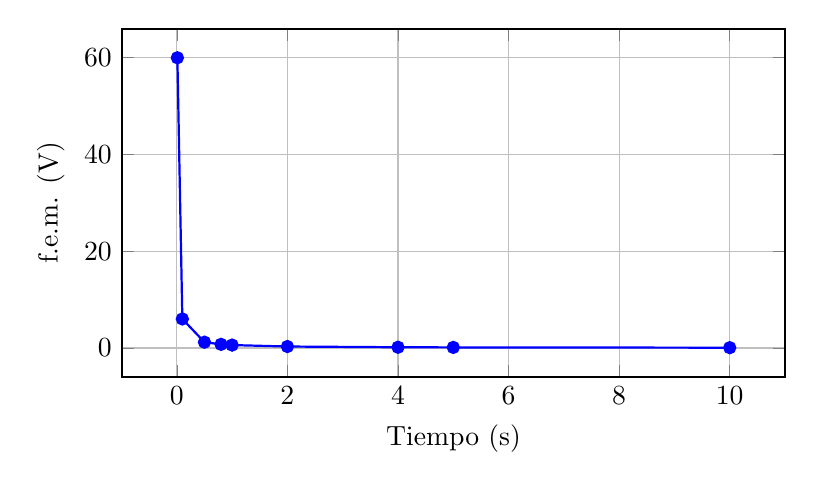
\begin{tikzpicture}
\begin{axis}[
    xlabel={Tiempo (s)},
    ylabel={f.e.m. (V)},
    width=10cm, height=6cm,
    grid=both,
    thick
]
\addplot[mark=*, blue] coordinates {
    (0.01, 60)
    (0.1, 6)
    (0.5, 1.2)
    (0.8, 0.75)
    (1, 0.6)
    (2, 0.3)
    (4, 0.15)
    (5, 0.12)
    (10, 0.06)
};
\end{axis}
\end{tikzpicture}
\end{center}

\noindent\textbf{9.} Una bobina de $N=200$ espiras se mueve cortando perpendicularmente un campo magnético. La variación de flujo experimentado es uniforme y va desde los $\Phi_1=\qty{5}{mWb}$ a los $\Phi_2=\qty{10}{mWb}$ en un intervalo de tiempo de $\Delta t = \qty{0,5}{s}$. Averiguar la f.e.m inducida.

\begin{align*}
\text{fem} = N \cdot \frac{\Delta \Phi}{\Delta t} &= 200 \cdot \frac{\qty{0,01}{Wb} - \qty{0,005}{Wb}}{\qty{0,5}{s} - \qty{0}{s}} \\
&= 200 \cdot \frac{\qty{0,005}{Wb}}{\qty{0,5}{s}} = 200 \cdot \qty{0,01}{V} = \boxed{\qty{2}{V}}
\end{align*}

\noindent\textbf{10.} Una bobina de $N=100$ espiras corta con un ángulo de $45^\circ$ un campo magnético uniforme, la variación de flujo experimentada es uniforme y es de $\Delta \Phi = \qty{4}{mWb}$ en $\Delta t = \qty{1}{s}$. Averiguar la f.e.m inducida.

\begin{align*}
\text{fem} = N \cdot \frac{\Delta \Phi}{\Delta t} &= 100 \cdot \frac{\qty{0,004}{Wb}}{\qty{1}{s}} \\
&= 100 \cdot \qty{0,004}{V} = \boxed{\qty{0,4}{V}}
\end{align*}

\noindent\textbf{11.} Los terminales de una bobina son conectados a una resistencia $R=\qty{1}{\Omega}$ y se genera una corriente de $I=\qty{0,5}{A}$ y cuando esta se mueve produce una variación de flujo de $\Delta \Phi =\qty{5}{mWb}$ en $\Delta t = \qty{2}{s}$ ¿Cuántas espiras N tiene?

Sabemos que $V = R \cdot I$ y también que $V = N \cdot \frac{\Delta \Phi}{\Delta t}$. Igualando ambas expresiones:
\begin{align*}
R \cdot I &= N \cdot \frac{\Delta \Phi}{\Delta t} \\
N &= \frac{R \cdot I \cdot \Delta t}{\Delta \Phi} = \frac{(\qty{1}{\Omega}) \cdot (\qty{0,5}{A}) \cdot (\qty{2}{s})}{\qty{0,005}{Wb}} = \frac{\qty{1}{V \cdot s}}{\qty{0,005}{Wb}} = \boxed{200 \text{ espiras}}
\end{align*}

\noindent\textbf{12.} Hallar la longitud que tiene que tener un conductor que corta perpendicularmente un campo magnético el cual posee una inducción de $B=\qty{3}{T}$, y moviéndose a una velocidad de $v=\qty{5}{m/s}$ genera una f.e.m de $e=\qty{10}{V}$.

\begin{align*}
\epsilon = B \cdot l \cdot v \Rightarrow l &= \frac{\epsilon}{B \cdot v} \\
l &= \frac{\qty{10}{V}}{(\qty{3}{T}) \cdot (\qty{5}{m/s})} = \frac{\qty{10}{V}}{\qty{15}{T \cdot m/s}} = \boxed{\qty{0,66}{m}}
\end{align*}

\end{document}